\documentclass[usenames, dvipsnames, twocolumn]{article}      % article class
\usepackage[utf8]{inputenc}


\newcommand{\mytitle}{A Hybrid Physical \& Statistical Approach to Storm Surges}
\newcommand{\penname}{Candidate 8205R}
\newcommand{\supervisor}{\\Supervisor:\\  Dr. Dan Jones,\\ British Antarctic Survey}


\usepackage{Theme/mystyle}
\usepackage{Theme/globals}
% Define some vital globals for the document etc.

% Where I put the images to be imported.
\graphicspath{{images/}{../images/}}

\addbibresource{references/generic_references.bib}
\addbibresource{references/references.bib}
\addbibresource{references/fluid_dynamics.bib}
\addbibresource{references/machine_learning.bib}
\addbibresource{references/global_warming.bib}
\addbibresource{references/programming.bib}
\addbibresource{references/surge.bib}
\addbibresource{references/tebbutt.bib}
\addbibresource{references/taleb.bib}
\addbibresource{references/evt.bib}
\addbibresource{references/cyclone.bib}
\addbibresource{references/meteorology.bib}
  % bibliography added here

\usepackage{cleveref}
% I prefer the automatic § symbol when I'm referencing sections.
\crefformat{section}{§#2#1#3}
\crefformat{subsection}{§#2#1#3}
\crefformat{subsubsection}{§#2#1#3}

\setlength\headheight{26pt} %% just to make a warning go away.
\rhead{\thepage}  % right head page number.
% page number on right head
\lfoot{\penname}  % left foot author.
\cfoot{}
\rfoot{}
\pagestyle{fancy}  % use fancyhdr style

\date{\today}
\title{\vspace*{-100pt}\textbf{\mytitle}\vspace{-0pt}}
\newcommand\thanksmessage{Thanks to Dr.~Laure Zanna (New York University) [advice and co-supervision],
Dr.~Pierre Mathiot (Met Office) [data],
and Dr.~Rory Bingham (Bristol) [advice].
None of these have seen this thesis; any mistakes are my own.}
\author{\penname\thanks{\thanksmessage } \\  \supervisor }
\newcommand\words{4921}
\newcommand\pages{22}
\newcommand\abwords{150}

\usepackage{moreverb} % for verbatim ouput
% Count of words
\immediate\write18{texcount -nc -inc -merge -sum -q report.tex > wordcount/wordcount.tex}
\newcommand\wordcount{ \verbatiminput{wordcount/wordcount.tex}}

%%%%%%%%%%%---Actual Document---%%%%%%%%%%%%%%%%%%%%%%%

\begin{document}

\iftrue

%TC:ignore


\section*{The effects of COVID19 on this thesis.}
\begin{itemize}

\item One person in my house caught had symptoms of COVID19, and so I had to self-isolate
      for the first period of 14 days.

\item I had to take care of my partner whilst
      they had a fever, and subsequently self-isolate for an additional 14 days.

\item We both lived and worked in around 9 m$^{2}$ of floor space, which is not as
      good a work environment as an office.

\item I was less able to collaborate with other members
      of the British Antarctic Survey due to not being in the office.

\item Some of my notes, and my official lab-book were locked into my BAS office when full lockdown was declared,
      as I only had access to a small amount of car space to bring my material back.
      I therefore had to find similar material elsewhere. This wasn't a serious inconvenience,
      but it did waste some time. Perhaps this was my fault for not seeing where government policy was going.

\item I had the misapprehension that the lockdown would have ended in time for me to
      reclaim my official lab-book before hand in.

\item Having said all this, I was mainly able to carry on as normal because
      my work is computer-based, and so I was much less impacted than an experimentalist.
      Without this project to do, lockdown would have been much less tolerable,
      and I am proud of the work that I managed to finish.

\item I was also lucky to be able to able to present to in the CEDSG-AI4ER series
      the week before the first lockdown measures were put in place, and
      I found the feedback the audience gave very helpful.

\item My supervisor Dr.~Dan~Jones was also supportive,
      and we continued to have supervisory meetings over zoom,
      sometimes with Dr.~Laure~Zanna (NYU), and these provided some much
      needed structure.

\end{itemize}

[Non COVID related problems are discussed in the `deadends' section of the
appendix to this thesis.]

\newpage
[column left intentionally blank]

\newpage

[page left intentionally blank]
\newpage

\subfile{sections/Title_Page}
\fi
\iftrue
 \twocolumn[
  \begin{@twocolumnfalse}
  \maketitle
  \setcounter{page}{1}
    \begin{abstract}
    Storm surges are hazardous for life and property.
     I propose a new set of methods whereby they can be studied
     within an arbitrary climate model without inundation;
     I introduce simple algorithms for selecting coastlines,
      with two new metrics for the bathymetry and convexity of the coast.
       These are tied to two new metrics for the responsiveness of a coastline point to the sea stress state,
        where the relationship is static between coastlines in an ORCA12 NEMO hindcast of 2004-5.
        Finally I use the potential intensity theory of hurricanes, combined with extreme value theory,
        for a 101-year experiment (\texttt{control-1950}, ORCA12, HadGEM3)
        show that the there is a reasonable potential method for combining physical
        and statistical knowledge to better estimate hazards,
        although this requires further testing. This should provide
        a strong basis for future work applying these
        methods to the ensemble of global climate models,
        and incorporating observational data.


    % \paragraph{Keywords:} \textit{Tropical Cyclones (TCs),
    %                              Physically Limited Extreme Value Theory (EVT),
    %                              Warped Gaussian Processes (GPs),
    %                              Machine Learning (ML).
    %                              }
    \end{abstract}
    \vspace{20pt}
  \end{@twocolumnfalse}
]


%TC:endignore

%%%%%%%%%%%---Real Report---%%%%%%%%%%%%%%%%%%%%%%%%%%%

\section{Introduction}
\label{sec:1_Introduction}


Storm surges are coastal sea levels which far exceed those
expected given the tide.
They are caused by tropical cyclones
(TCs) and extratropical cyclones (ECs).
TCs draw their kinetic energy from the thermodynamic disequilibrium between
the tropical sea surface and the troposphere~\cite{emanuel1986air, emanuel1987dependence},
whereas ECs draw theirs from the
polewards temperature gradient~\cite{lorenz1960energy, holton2004introduction}.\footnote{
This is technically called baroclinic instability.}
Their respective names reflect that conditions favourable
to their formation and growth are within and without the tropics respectively.\footnote{
Practically they are differentiated using algorithms like \texttt{TSTORMS}
\url{https://www.gfdl.noaa.gov/tstorms/} as in Y20~\cite{ZannaPreprint}.}
Because they have lower central pressures and sustain greater winds,
TCs create more dangerous storm surges~\cite{emanuel2005divine}.

TCs have historically been the
world's largest physical hazard~\cite{shultz2005epidemiology},
for economic damage,
and specifically TC storm surges for lives lost~\cite{shultz2005epidemiology,
zhang2009tropical, emanuel2005divine}.
This hazard is increasing as more people live on vulnerable coastlines
in insufficient buildings~\cite{emanuel2005divine}.
Anthropogenic climate change (ACC) is expected to exacerbate this,
as it begins to increase the maximum TC intensity\footnote{
However the uptick in TCs is not currently above
 natural variability~\cite{mendelsohn2012impact}.}
(see~§~\ref{sec:hurr-theory})~\cite{emanuel2008hurricanes,emanuel2017will},
and to sea level rise placing more areas at risk~\cite{SROCC}.
The range of hurricanes may also increase~\cite{fedorov2010tropical}.

Quantifying how this hazard will change is necessary
so that the public can act with foresight.
Others have already begun to apply machine learning (ML) techniques to this
end~\cite{kulp2019new, kulp2018coastaldem, tadesse2020data}.



\begin{table}[ht]
\resizebox{\columnwidth}{!}{%
\begin{tabular}{l L{6.5cm}}

\hline \hline
\textbf{Ab} & \textbf{Expansion}\\
\hline
EVT & Extreme value theory \\
GEV & Generalised extreme value (distribution) \\
BM & Block maxima \\
ML & Machine learning \\
GP & Gaussian process \\
TC & Tropical cyclone \\
EC & Extratropical cyclone \\
CMIP & Coupled model intercomparison project \\
Y20 & Yin et al.~2020~\cite{ZannaPreprint} \\
T19 & Taleb 2019, \textit{The Statistical Consequences of Fat Tails}~\cite{taleb2019statistical}\\
SSH & Sea surface height above geoid (m) \\
SST & Sea surface temperature ($^{\circ}$C) \\
\texttt{tyr} & \texttt{two-year} 2004-5 hindcast (§~\ref{sec:rean-prod}) \\
\texttt{c50} & \texttt{control-1950} experiment (§~\ref{sec:control-1950-intro}) \\
\texttt{vc} & N-Vietnam \& China coastline (§~\ref{sec:coast-sample})\\
\texttt{eUS} & East US coastline (§~\ref{sec:coast-sample})\\
\hline \hline
\end{tabular}
}
\caption{Abbreviations (Ab) used in this report.}
\label{tab:abb}
\end{table}


This thesis begins to develop new methods of achieving this goal
as inspired by Yin~et~al.~2020~\cite{ZannaPreprint} (henceforth Y20).
Initially, by developing algorithms for extracting the coastlines from climate models
and metrics to characterise that coastline in §~\ref{sec:coast}.
Developing from Y20~\cite{ZannaPreprint}, I compare measures for the
responsiveness of a stretch of the coastline to wind stress.
I show using extreme value theory (EVT), that the
distributions of extreme events are controlled by the same factors as
the responsiveness under normal circumstances.
Finally, I suggest a
method of improving a naive EVT fit, using our physical knowledge
of the thermodynamic limit
to the maximum intensity of a hurricane~\cite{emanuel1999thermodynamic}
 given a climate (see~§~\ref{sec:hurr-theory})~\cite{emanuel1987dependence,
 emanuel2016predictability}.
I discuss the merits and deficiencies of these,
and suggest how they could be built upon in future work (§~\ref{sec:future}).

%\FloatBarrier
\fi
\iftrue
\section{Background}
\subsection{Model Experiments}
\subsubsection{NEMO models}
\paragraph{Introduction}
\label{sec:nemo}
I was able to use two outputs~§~\ref{sec:rean-prod}~\&~§~\ref{sec:control-1950-intro}
of use the NEMO ocean engine~\cite{madec2015nemo}, which uses the tripolar ORCA12 grid,
with a  $\frac{1}{12}^{\circ}$
resolution, designed so that no coordinate singularities are in the ocean~\cite{madec1996global}.


 The bathymetry is from
 ETOPO2v2~\cite{lecointre2011definition, noaa20062}.\footnote{\url{https://www.ngdc.noaa.gov/mgg/global/etopo2.html}}
 This is more accurate along the US coastline, using
 direct measurements rather than altimetry data~\cite{noaa20062}.
 Table~\ref{tab:mod-symb} introduces the variables taken from NEMO.




\begin{table}[ht]
\resizebox{\columnwidth}{!}{%
\begin{tabular}{l L{5.5cm} l}

\hline \hline
\textbf{Sym} & \textbf{Name} & \texttt{cn}\\
\hline
$\eta$ & SSH & \texttt{zos} \\
$\tau_u$ & Sea surface stress along u (Pa) & \texttt{tauuo} \\
$\tau_v$ & Sea surface stress along v (Pa)& \texttt{tauvo} \\
$|U|$ & Surface Ocean Windspeed (m s$^{-1}$) & \texttt{sowindsp}\\
\hline \hline
\end{tabular}
}
\caption{Symbols (sym), names and \texttt{code-names} (\texttt{cn})
taken from NEMO outputs in this report.}
\label{tab:mod-symb}
\end{table}


\paragraph{Limitations}

Neither output
include tides, inundation, or wave setup.
The resolution means that cells are around
8km wide, therefore the sea surface height (SSH)
is recorded around 4km from the coast.

\subsubsection{2004-5 \texttt{two-year} hourly reanalysis product}
\label{sec:rean-prod}
Dr.~Pierre Mathiot kindly ran a global ocean model with
hourly outputs for 2004-5 (\texttt{tyr}) (see Figure~\ref{fig:katrina}).

\paragraph{EN4 initial conditions}
EN4 is a reanalysis product, starting in 1976,
 that uses all available ocean profiles~\cite{good2013en4, HadObs}
to produce a best guess as to what the properties of the ocean are.


\paragraph{CORE2 forcing}
CORE2 is a set of global air-sea fluxes in 6 hour time steps which are interpolated between~\cite{griffies2012datasets,large2009global,
 hurrell2008new}\footnote{\url{https://climatedataguide.ucar.edu/climate-data/corev2-air-sea-surface-fluxes}}
 (see Figure~\ref{fig:katrina}B-D).
 These were made from the a reanalysis product,
 bias corrected with satellite data~\cite{core2, core2expert}.


\begin{figure}[htb!]
\centering
\includegraphics[width=\linewidth]{../surge/plots/katrina_graph.pdf}\\
\vspace{-9pt}
\includegraphics[width=\linewidth]{../surge/plots/new_orleans_map.pdf}
\caption{The landfall of Hurricane Katrina within \texttt{tyr}  from three points
 around New Orleans (NO). As shown in D, the eye of the TC
crosses passes through this area. The wind stresses experienced at the
the three points are similar (B~\&~C), but the response (A) is much
less significant at the headland than the other two points.
B-D are consistent with CORE2's fields being interpolated from 6~hour
steps as in~\cite{core2expert}.
The bearing angles are explained in §~\ref{sec:convexity}.
}
\label{fig:katrina}
\end{figure}


\subsubsection{\texttt{control-1950} daily means}

\label{sec:control-1950-intro}

The second source of data was the \texttt{control-1950} HadGEM3 experiment (\texttt{c50}),
made available via the PRIMAVERA project.
The HadGEM3 coupled climate model~\cite{williams2018met, FurtherInfo},
 was the Met Office's submission to CMIP6,
although \texttt{control-1950} is not a standard CMIP6 experiment~\cite{eyring2016overview}
.\footnote{CMIP is the coupled model intercomparison program,
whose models form part of the scientific basis for the IPCC
reports (e.g.~\cite{SROCC}).}

\texttt{control-1950} has its forcing kept at
1950s levels for 101 360-day years. Outputs are recorded as daily
means~\cite{williams2018met, FurtherInfo}.\footnote{\url{https://view.es-doc.org/
        ?renderMethod=name&project=cmip6&type=cim.2.designing.NumericalExperiment&client
        =esdoc-url-rewrite&name=control-1950}}
Due to time constraints, and varied model grids, only the SSH outputs were used in this report.


\FloatBarrier
\fi


\section{Coastlines within a climate model}
\label{sec:coast}
\subsection{Selection}
 \subsubsection{Fractal coastline}
 \label{sec:fractal}
 The coastline appears to be a self-similar fractal~\cite{mandelbrot1967long,
 richardson1961problem}, by which is meant that it has the same features at all
 scales, so that the length of the coast increases without limit as resolution
 is increased.
 A consequence of this is that a coastline has no defined length without
 reference to the resolution at which it is measured.
 This presents some problem when comparing different climate models as they will have different
 numbers of coastal cells. It has been observed that the fractal dimension changes
  along the East US coast~\cite{jiang1998fractal}
 and this would mean that the relative number of coastal cells between different
 points will also change as the resolution is increased.

\subsubsection{Algorithms}
\label{sec:coast-algorithms}
Algorithms~\ref{algo:Selection}~\&~\ref{algo:Sort} first extract the coastline
from the surface slice of the ocean field and then pick out a single chain of
coastal points between two chosen ends. The list of points can be further
manually sorted to remove unwanted regions such as large bays (e.g.~Chesapeake~bay)
and the occasional river island (e.g.~Shanghai bay's island). Once this is
done \texttt{xarray} can be used to quickly extract these points
from the climate model to make a new NetCDF file.



\begin{algorithm}[H]
\dontprintsemicolon
% \DontPrintSemicolon % Some LaTeX compilers require you to use \dontprintsemicolon instead
\caption{Coastal Selection}
\label{algo:Selection}
\KwIn{Grid: boolean grid (True for NaN values (land))}
\For{indices in Grid}{
  \If {Grid[indices] == False}{
     \If{ any of Grid[index\_x $\pm$ 1, index\_y $\pm$ 1] are True}
        {\textbf{append} indices to List\;}
     }
}
\KwOut{List: list of indices}
\end{algorithm}

\begin{algorithm}[H]
\dontprintsemicolon
% \DontPrintSemicolon % Some LaTeX compilers require you to use \dontprintsemicolon instead
\caption{Coastal Sort}
\label{algo:Sort}
\KwIn{Input\_List: Slimmed output of Algorithm~\ref{algo:Selection}}
\KwIn{First\_Index\_Pair: Point at one end of the coast }
\KwIn{Final\_Index\_Pair: Point at other end of the coast }

\texttt{tmp} $\gets$ First\_Index\_Pair\;

\Repeat{\texttt{tmp} = Final\_Index\_Pair}{
 \textbf{append} \texttt{tmp} to Output\_List\;
 \textbf{remove} \texttt{tmp} from Input\_List\;
 \texttt{tmp} $\gets$ Input\_List[\textbf{min}$_{k}$(\textbf{distance}(\texttt{tmp}, Input\_List[k]))]\;
}
\textbf{append} Final\_Index\_Pair to Output\_List\;

\KwOut{Output\_List: sorted list of indices}
\end{algorithm}


\subsubsection{Sample coastlines}
The first coastline chosen was the eastern coastline of the mainland
United States, so that it could be compared with~\cite{ZannaPreprint},
and because the topography of the NEMO models is most accurate along the
US coastline.

Secondly I extracted the coastline from Hue, Northern Vietnam, to China's
border with North Korea, removing Shanghai bay island.

Finally we extracted the eastern coastline of Honshu island, Japan.

\subsection{Metrics}
\subsubsection{Motivation}
A quick look at the coast revealed that certain features stuck out:
high kurtosis at New Orleans (NO), at the end of a shallowly sloping bay;
low kurtosis at Miami (MM), at the end of the headland of Florida.
But it would be interesting to find out what is really the controlling
factor, or whether either of these are truly predictive of storm surge risk.

To assess this question, it is necessary to quantify these two coastal attributes
and given that the coast is fractal (§~\ref{sec:fractal}), these metrics must also be defined at
all scales.

\subsubsection{Convexity}
Given a selected coastline, we have a list of points of latitude and longitude.
We can define the normal bearing to the coast.

This provides a convexity value for every smoothing length $\sigma$.

\subsubsection{Bathymetric gradient}
The simplest way of working this out is to look at the
bathymetry netCDF file that the model was run with (ETOPO2v2-derived in this
 case (§~\ref{sec:nemo})), and work out where some set of chosen isobaths are.
Once these isobaths have been selected, the cartesian distance
within the model grid from every point on
the coast to that isobath are calculable.

This provides a distance-to-isobath value for each of the isobaths
queried.


\iftrue
\section{Preprocessing coastal data}
The sea surface height in the model is relative to
a reference geoid: the surface that a homogeneous static fluid would occupy
on an azimuthally symmetric Earth of the same size and rotation frequency.
Dynamic topography emerges because of the
currents and density contrasts (Figures~\ref{fig:zos}~\&~\ref{fig:ssh_stats_america}A).

\begin{figure}
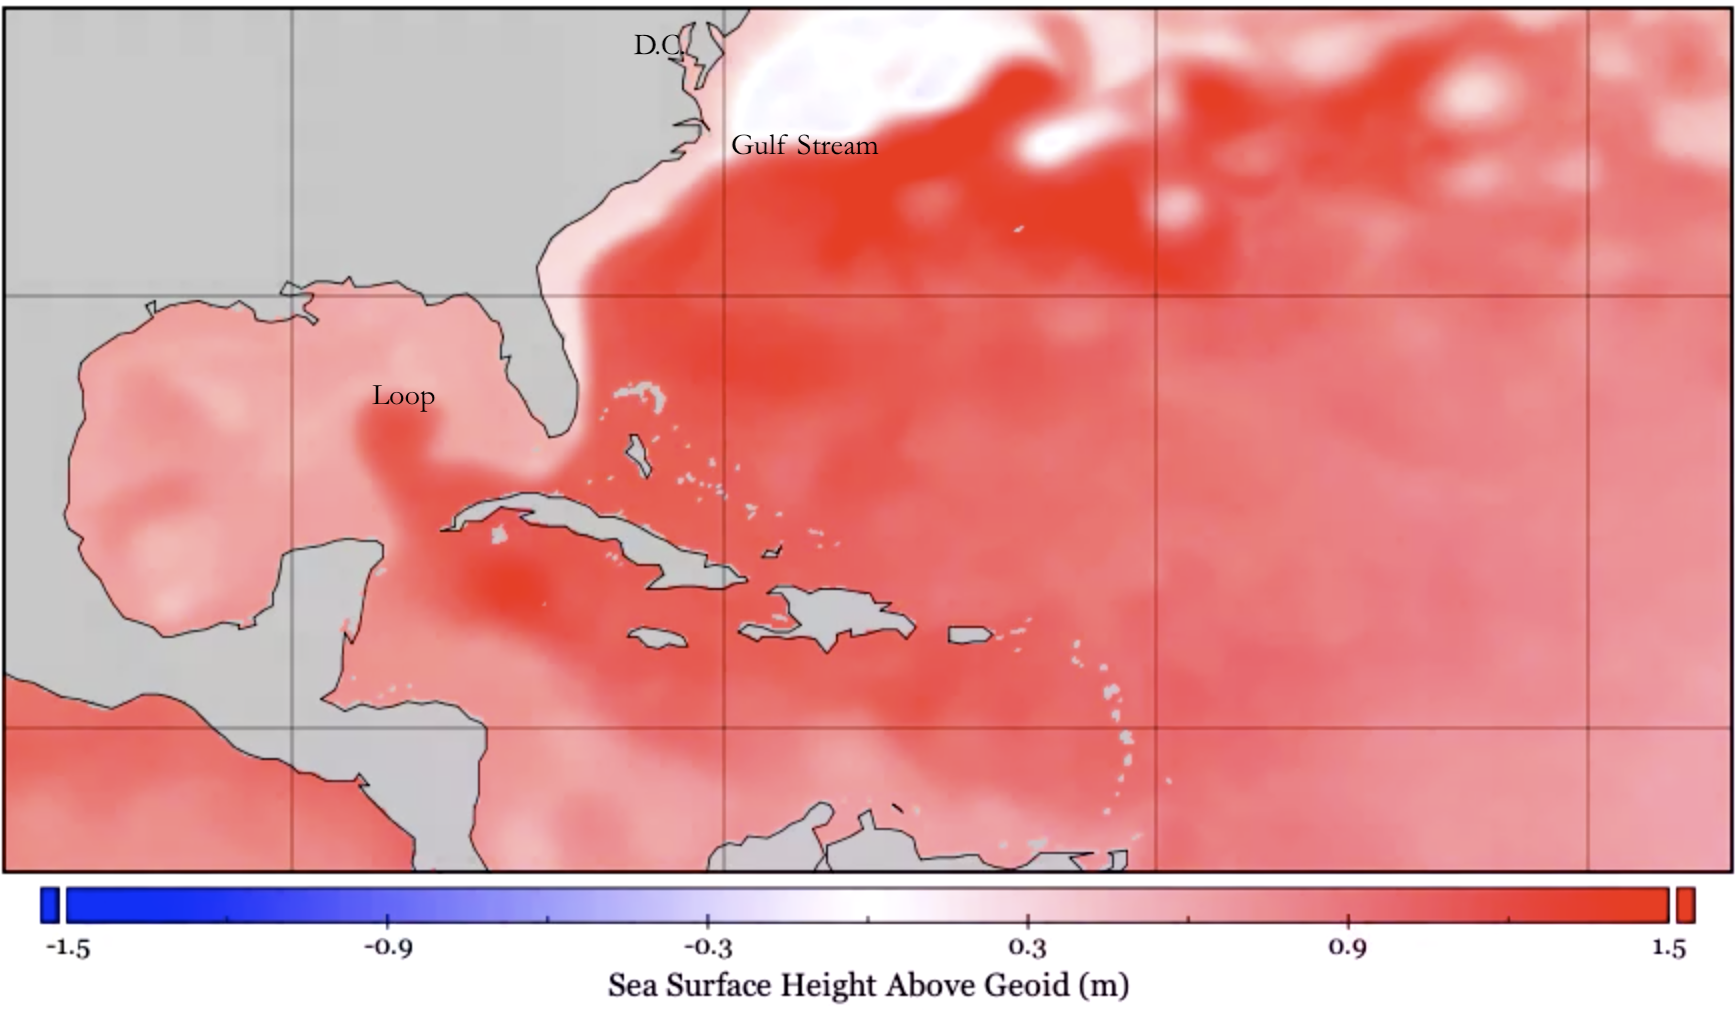
\includegraphics[width=\linewidth]{images/example-images/zos-image.png}
Sea Surface Height above Reference Geoid (\texttt{zos}, $\eta$, SSH)
\label{fig:zos}
\end{figure}




We define the third  moment around the mean,

\begin{equation}
\operatorname{Skew}[X]\equiv \mathbb{E}\left[\left(\frac{X-\mu}{\sigma}\right)^{3}\right]
=\frac{\mathbb{E}\left[(X-\mu)^{3}\right]}{\left(\mathbb{E}\left[(X-\mu)^{2}\right]\right)^{3 / 2}},
\end{equation}

and fourth as the excess above the Gaussian~\cite{taleb2019statistical},

\begin{equation}
\operatorname{Kurt}[X]=
\mathbb{E}\left[\left(\frac{X-\mu}{\sigma}\right)^{4}\right]-3
\equiv \frac{\mathbb{E}\left[(X-\mu)^{4}\right]}{\left(\mathbb{E}\left[(X-\mu)^{2}\right]\right)^{2}}-3.
\end{equation}




\begin{figure*}[htb!]
    \centering
    \includegraphics[width=0.6\linewidth]{../surge/plots/stats_points_plot.pdf}
       \hspace{0pt} \includegraphics[width=0.285\linewidth]{../surge/plots/stats_points_plot_1.pdf}
    \vspace{-7pt}
    \caption{A comparison between the distributions of sea surface height, $\eta$ (SSH/zos).
     above geoid for 2005 (red) and 2004 (blue),
     with the Pearson correlation coefficient, $r_p$, for each moment between the two years in A--D.
     Kurtosis in frame D is the excess above that expected for a normal distribution,
     which shows that areas like NO are highly non-normal (a statistical test
     shows that the probability of it being sampled from a Gaussian is $<10^{-304}$)~\cite{anscombe1983distribution}.
     An artefact in the data is that the mean of all of the points for the coastline
     seems to be uniformly shifted upwards between the two years (A~\&~E),
     where the difference is $0.06\pm0.01$m. }
   \label{fig:ssh_stats_america}
\end{figure*}



These are useful to summarise the SSH statistics
for \texttt{eUS} in Figure~\ref{fig:ssh_stats_america}.\footnote{
The individual points' SSH (Figure~\ref{fig:individual_zos} in §~\ref{sec:sum-var-stat}),
do not reveal any discontinuity in the data in \texttt{tyr},
 but Figures~\ref{fig:four-trans-panels}-\ref{fig:mm-hp-lp}
suggest that the displacement might be caused by \texttt{tyr} spin up from the
initial conditions.
}
On the right of panels \ref{fig:ssh_stats_america}A--D
is the Pearson regression coefficient, $r_p$,
between the two years for that moment, which shows that the mean and
std~dev of a point are c.~static between the years,
but the higher order moments of skew and kurtosis
(\ref{fig:ssh_stats_america}~C~\&~D) are more sensitive to the
random incidence of storms on the coast.


\label{sec:fourier}

The Fourier transform is defined as,

\begin{equation}
F(f)=\int_{-\infty}^{\infty} y(x) e^{-i 2\pi f x} d x,
\end{equation}

which in discrete form~\cite{cooley1965algorithm} is,


\begin{eqnarray}
\sum_{n=0}^{N-1} a_{n} e^{-2 \pi i  k n/ N}=&\sum_{n=0}^{N / 2-1} a_{2 n}
e^{-2 \pi i k (2 n)/ N}  \\ &+\sum_{n=0}^{N / 2-1} a_{2n+1} e^{-2 \pi i k (2 n+1)/ N}. \notag
\end{eqnarray}

Fourier transforms of real signals have Hermitian symmetry,

\begin{equation}
\mathcal{F}{(-g(x))}=\mathcal{F}(g(x))^{*},
\end{equation}

implies that negative frequencies have no information not in the positive.


Figures~\ref{fig:zm_fft_zos}~\&~\ref{fig:zm_fft_tos} give the
Fourier transform spectrums of SSH and SST respectively.
Figures~\ref{fig:zm_fft_zos} shows that SSH has a red-noise spectrum,
which is true of the ocean in general, and Figure~\ref{fig:zm_fft_tos}
shows that SST is dominantly annual (as expected).
The relationship between the temperature and the sea surface temperature.
The Florida current is a likely source of particularly red noise at Miami
(Figures~\ref{fig:vos}~\&~\ref{fig:uos}).
The general eddy activity is visible in Figures~\ref{fig:vos}~\&~\ref{fig:uos}
as the loop current has formed a secondary vortex ring moving northwards
in Figures~\ref{fig:uos}~to~\ref{fig:vos}.
Figures~\ref{fig:no-hp-lp}~\&~\ref{fig:mm-hp-lp} show a high and
low pass filter applied to specific points, and Figure~\ref{fig:four-trans-panels},
which are defined as:


\Delta\eta_{\;\mathrm{lp}}(t) = \int_{\mathbb{R}}W\left(\frac{|f|}
{|f|_{\mathrm{thresh}}}\right)\int_{\mathbb{R}}e^{2\pi i (t-t^{\prime})f }
\Delta \eta(t^{\prime})dt^{\prime}df,
\end{equation}
\begin{equation}
\Delta\eta_{\;\mathrm{hp}}(t) = \int_{\mathbb{R}}\left(1-W\left(\frac{|f|}
{|f|_{\mathrm{thresh}}}\right)\right)\int_{\mathbb{R}}e^{2\pi i (t-t^{\prime})f}
   \Delta \eta(t^{\prime})dt^{\prime}df.
\end{equation}


\begin{figure}
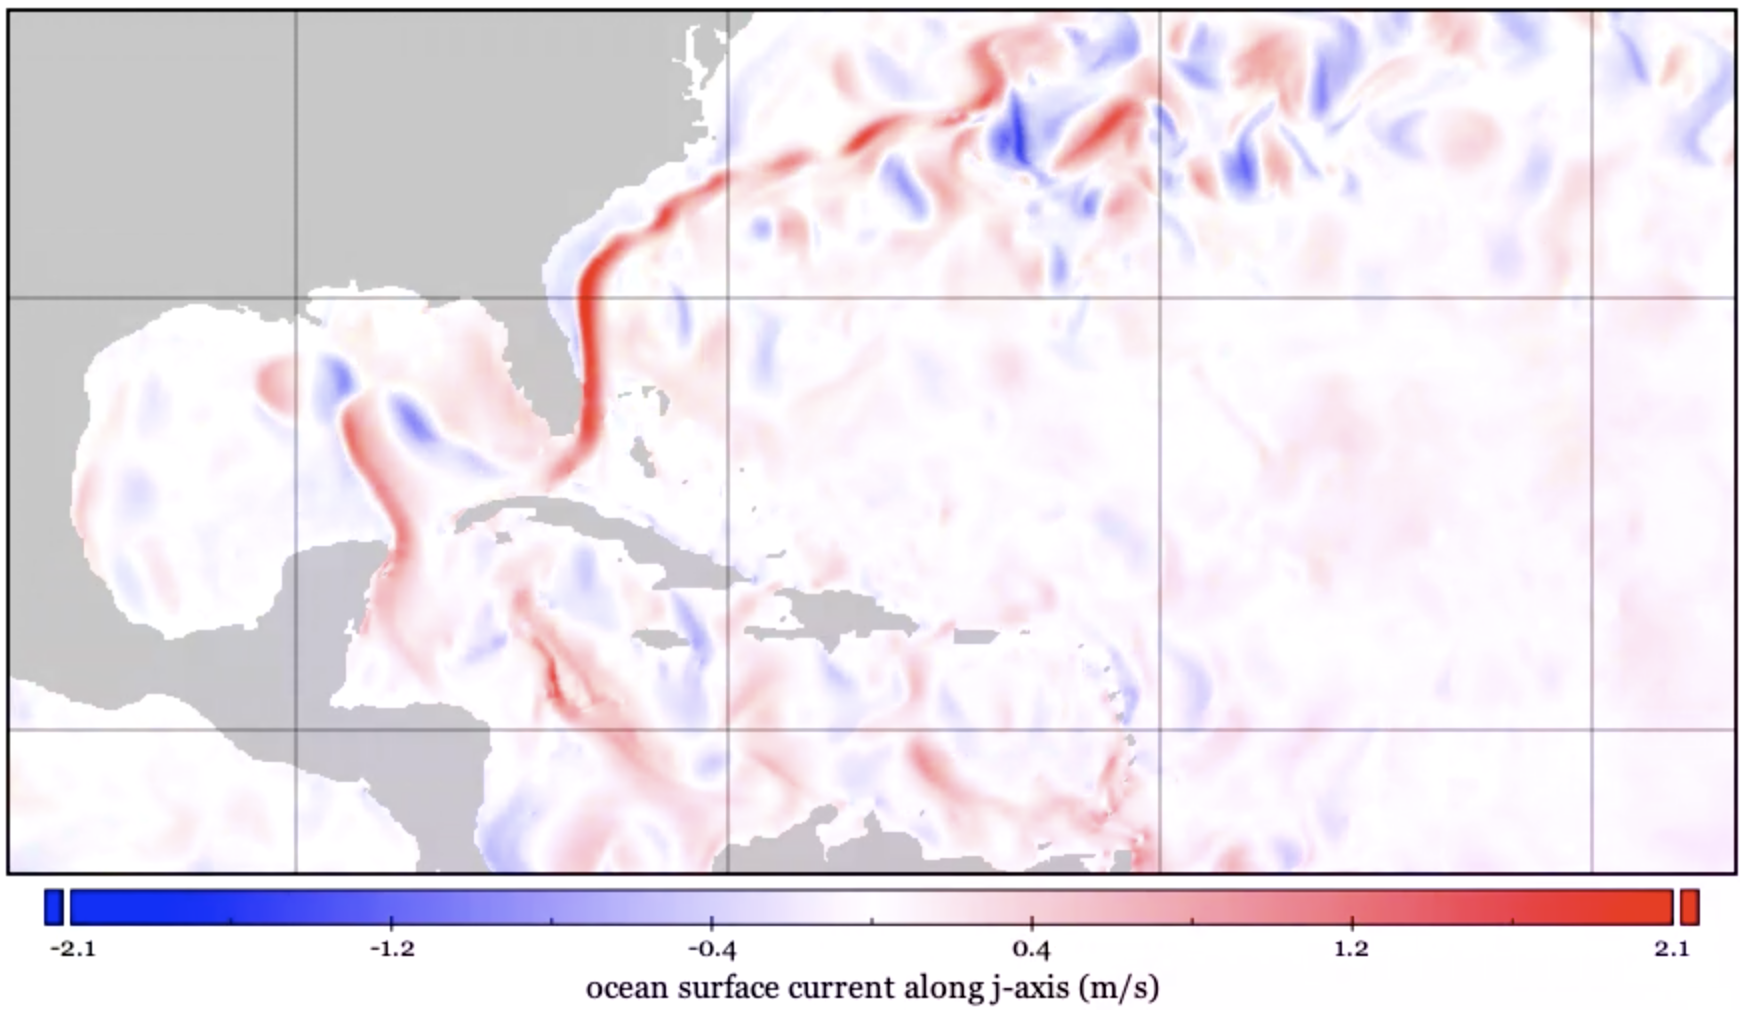
\includegraphics[width=0.93\linewidth]{images/example-images/vos.png}
\caption{Sea surface velocity along Y-axis, (\texttt{vos}, $v$)}
\label{fig:vos}
\end{figure}

\begin{figure}
\vspace{-10pt}
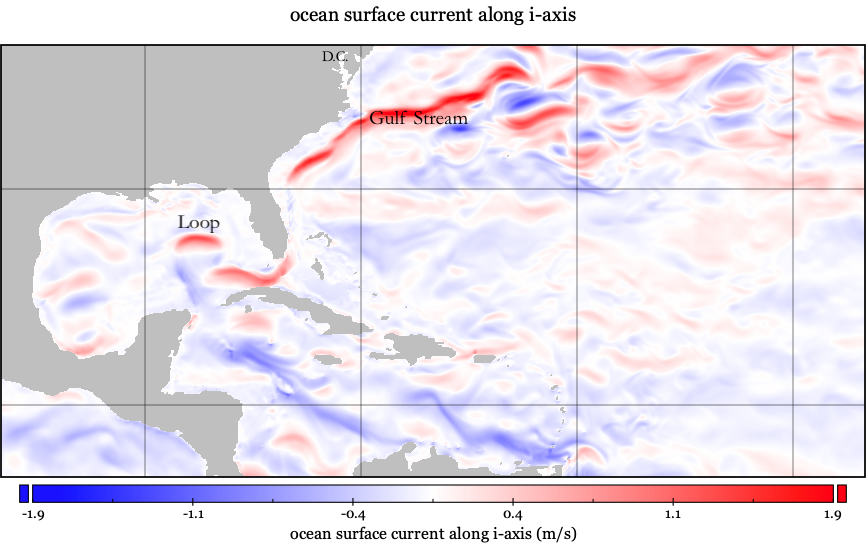
\includegraphics[width=\linewidth]{images/example-images/uos.png}
\caption{Sea surface velocity along X-axis,
         (\texttt{uos}, $u$) from \texttt{tyr}
         on 4th August 2005. }
\label{fig:uos}
\end{figure}



\begin{figure*}
\includegraphics[width=0.48\linewidth]{../surge/plots/low_pass_grid.pdf}
     \includegraphics[width=0.48\linewidth]{../surge/plots/high_pass_grid.pdf}
\caption{Fourier Transform~\cite{cooley1965algorithm} of SSH demeaned by
         coastal point, and low (left) and high (right) pass filtered respectively,
         with a threshold of 2 yr$^{-1}$ (justified by
         Figure~\ref{fig:lpredthresh}). Although not noticeably different in
         the low pass filter (left), Miami and other headlands
         are noticeably less variable in the high pass filter. }
\label{fig:four-trans-panels}
\centering
\includegraphics[width=0.8\linewidth]{../surge/plots/norlean-low-pass.pdf}
\vspace{-10pt}

\caption{New Orleans (NO) closest coastal cell divided
         into high and low frequency components.}
\label{fig:no-hp-lp}


\includegraphics[width=0.8\linewidth]{../surge/plots/mm-low-pass.pdf}
\vspace{-10pt}

\caption{Miami (MM) has more low frequency noise.
         Both this and Figure~\ref{fig:no-hp-lp} above
         show an increase in the low amplitude signal with time,
         which could be explained by the spin
         up of \texttt{tyr} from EN4.}
\label{fig:mm-hp-lp}

\end{figure*}



\begin{figure*}
\centering

\vspace{-35pt}
       \includegraphics[width=0.27\linewidth]{../surge/plots/reg_fft/up_to_100_full_coast.png}
        \includegraphics[width=0.35\linewidth]{../surge/plots/reg_fft/up_to_100_coastal_average.png}
            \caption{\texttt{eUS-tyr} An averaged $r^2$ between \texttt{huber} and \texttt{MLR} trained on 2004 and 2005,
                    and tested on the opposite year (see §~\ref{sec:responsiveness}).}
            \label{fig:lpredthresh}

\begin{minipage}{0.45\textwidth}
\includegraphics[width=1\linewidth]{../surge/plots/lag/fft_pp_zos.png}
            \includegraphics[width=\linewidth]{../surge/plots/lag/zm_fft_pp_zos.png}
            \caption{\texttt{eUS} for \texttt{tyr} demeaned SSH, $\Delta\eta$, fourier transform. Bottom plot is a zoomed in version of the upper.}
            \label{fig:zm_fft_zos}
            \end{minipage}\begin{minipage}{0.45\textwidth}

        \includegraphics[width=1\linewidth]{../surge/plots/lag/fft_pp_tos.png}
            \includegraphics[width=\linewidth]{../surge/plots/lag/zm_fft_pp_tos.png}
            \caption{\texttt{eUS} for \texttt{tyr} demeaned SST, $\Delta T_s$, fourier transform,
                     showing power c.~uniquely located in annual signal.}
            \label{fig:zm_fft_tos}
            \end{minipage}

\end{figure*}


\label{sec:lag}

\begin{figure*}
\includegraphics[width=1\linewidth]{../surge/plots/temp/ssh_sst_grid.pdf}
\caption{There is some interesting structure downstream of Miami, could this be
         movements in the Florida current?
         If so, could it be predictive of the SSH upstream}
         \label{fig:ssh-sst}

\centering
\includegraphics[width=0.45\linewidth]{../surge/plots/lag/correlate_dmdm.pdf}
         \caption{Lag correlation plot}
         \label{fig:lag-plot}
\end{figure*}


We would like to be able to explain this seasonal cycle in SSH.
The obvious choice would be to look at SST and SSH, as in Figure~\ref{fig:ssh-sst}
for \texttt{eUS} for \texttt{tyr}, and do lag correlation, which is defined as:

\begin{equation}
r_{k}=
\frac{\sum_{i=1}^{N-k}\left(X_{i}
-\bar{Y}\right)\left(X_{i+k}-\bar{Y}\right)}
{\sum_{i=1}^{N}\left(X_{i}
-\bar{Y}\right)^{2}}.
\end{equation}

Figure~\ref{fig:lag-plot} (\texttt{eUS}, \texttt{tyr}) tells a simple story of
SSH lagging slightly behind SST, as the mixed layer takes longer
to heat up than the surface.
However Figure~\ref{fig:vc_lag-plot} undermines this as the
lag becomes anti-phase, falsifying this simple hypothesis as
being generally true.
I suggest that Figure~\ref{fig:lpredthresh} justifies removing the low frequency
component of the signal, as it supports the hypothesis that the
low frequency signal cannot be predicted by sea surface stress.

\FloatBarrier

\section{Simple measures of responsiveness}
\label{sec:3_ORCA12_REG.tex}
\subsection{Linear ML models}
\label{sec:lin-ml-models}

To regress some set of inputs, $X$, against
some set of targets, $Y$,
we need to choose an objective function to minimise:

\begin{align}
J_{\mathrm{mlr}} = & \|X w-y\|_{2}^{2} \tag{MLR}, \label{eq:MLR} \\
J_{\mathrm{lasso}} = &
\frac{1}{2 n_{\text {samples }}}\|X w-y\|_{2}^{2}+\alpha\|w\|_{1} \tag{LAS}, \label{eq:LAS} \\
J_{\mathrm{ridge}} = &  \|X w-y\|_{2}^{2}+\alpha\|w\|_{2}^{2} \tag{RID}, \label{eq:RID}
\end{align}

Where \ref{eq:MLR} is the ordinary minimisation of least squares, that has no
penalty for the complexity of parameters.
The lasso objective function adds a penalty~\ref{eq:LAS},
$\alpha\|w\|_{1}$ added, where $\alpha$ is a constant and $\|w\|_{1}$ is the
$l_1$-norm of the coefficient vector.
The ridge objective function~\ref{eq:RID}
$\alpha\ge0$ controls the amount of shrinkage:
the larger value of $\alpha$,
the greater the amount of shrinkage
and thus the coefficients become more robust to multi-colinearity.
A coordinate descent algorithm is used to~\cite{scikit-learn}
$
\min _{w} (J)
$.

The complexity parameter $\alpha$, can be set to
the value that leads to the greatest generalisability to unseen data.


As shown in Figure~19~of~T20~\cite{ZannaPreprint}.
The threshold could be arbitrary,
so I chose that the SSH has to be greater than zero,
as it approximately guarantees that the sea surface stress is acting into
the coast rather than away from it.


\subsection{$\tau_u$, $\tau_v$ responsiveness}
\label{sec:tau-tau}
This method is quite crude, and could be simply improved.
Figure~\ref{fig:tau-tau-r-no} shows a single example of working out the linear
responsiveness (or linear predictability).
Figure~\ref{fig:tau-tau-resp} shows that when this same metric is applied along \texttt{eUS}
for each year in \texttt{tyr}. Figure~\ref{fig:tau-tau-responsiveness} creates a metric for the
responsiveness.



\begin{figure*}
\centering
 \hspace{-40pt} \includegraphics[width=0.6\linewidth]{../surge/plots/rmlr.pdf}
  \vspace{-15pt}
 \caption{A four panel plot to show the estimation of responsiveness
          of $\Delta\eta_{\mathrm{hp}}$ to $\tau_u$ and $\tau_v$, with the
          \texttt{MLR} and \texttt{Huber} algorithms. The y-units of A~\&~B are
           m Pa$^{-1}$.}
 \label{fig:tau-tau-resp}
 \hspace{-40pt} \includegraphics[width=0.3\linewidth]{../surge/plots/reg_angle.png}
  \vspace{-15pt}
 \caption{This shows that for the majority of the coastline there is a close
 corresponce between the normal bearing of the coast and the regression line ($r_p=0.83\pm0.05$).
 \texttt{np.arctan2(c0, c1)}}
  \label{fig:tau-tau-angle}
  \hspace{-40pt} \includegraphics[width=0.5\linewidth]{../surge/plots/adj_reg_mag.pdf}
   \vspace{-15pt}
  \caption{A more robust measure of responsiveness magnitude.
  ($\bar{r^2}$)\texttt{*np.sqrt(np.square(c0) + np.square(c1))}. }
   \label{fig:tau-tau-responsiveness}
\end{figure*}


\label{sec:angle}

Figure~\ref{fig:tau-tau-angle} shows that the angle is highly correlated with
the bearing of the coast that was defined in §~\ref{sec:convexity}.
The bearing of the regression line can be simply calculated,
and compared to the bearing of the normal coastline.
As shown, there is a systematic offset between the two lines,
which changes between them. This can be explained through the
classic theory of Ekman transport of the water.
Ekman~\cite{hope2013hindcast}.


\label{sec:reg-metrics}

The magnitude of this regression line varies in approximately the same
way for both methods, showing that there is some underlying property of the
coastline that both illuminate. In the previous section, I outlined
a series of metrics.

\label{sec:generalisability}

It would be possible that this is a spurious structure, where the fit
is made possible by giving so many information-less channels to fit against.
Therefore we need to use the other coasts to compare this against.
We use the Japanese and Chinese coast.

\begin{figure}[htb!]
    \centering
    \includegraphics[width=0.7\linewidth]{../surge/plots/ridge_lasso.pdf}
    \vspace{-15pt}
   \caption{\texttt{eUS} regression learning.
    Although not for lasso, and the regression is not consistent.
            We also need another coast to see if this generalises.}
    \label{fig:learnt-eus}

    \centering
    \includegraphics[width=0.8\linewidth]{../surge/plots/vc_ridge_lasso.pdf}
    \caption{The same as above, but for the \texttt{vc} coastline.}
    \label{fig:learnt-vc}
\end{figure}




\FloatBarrier

%\FloatBarrier
\section{Extreme value theory}
\label{sec:5_Transform}
\subsection{Idealised statistical theory}
The central limit theorem is a well known triumph of classical statistics,
and it is often useful in the physical sciences where the central value
is that of interest. However, by its nature the mean SSH will
not be able to damage the coast, and life and property will only be put
at risk by the most extreme events.

Extreme value theory is the provides the extension of this theory
to look at the return period of extreme events of a certain value.

Both require domain of attraction condition~\cite{bucher2018horse}:

\begin{enumerate}
  \item Either $\forall r \in \mathbb{N} \;\exists \;b_r \in \mathbb{R},\; \gamma\in \mathbb{R},\; a_r>0: $
    \begin{eqnarray}
    \lim _{r \rightarrow \infty} F^{r}\left(a_{r} x+b_{r}\right)=\exp \left\{-(1+\gamma x)^{-1 / \gamma}\right\} \\
     \text { for all } 1+\gamma x>0
    \tag{BM}
    \end{eqnarray}

  \item Or equivalently, there exists a positive function $\psi=\psi (t):$
    \begin{eqnarray}
    \lim _{t \uparrow x^{*}} \frac{1-F(t+\psi(t) x)}{1-F(t)}=(1+\gamma x)^{-1 / \gamma} \\
    \text { for all } 1+\gamma x>0
    \tag{POT}
    \end{eqnarray}
 \end{enumerate}

Normal Choices are POT or Block Maxima, but these strategies require
large amounts of data to converge~\cite{taleb2019much}.

BM leads to Generalised Extreme Value (GEV) distribution,
      whereas POT leads to Generalised Pareto Distribution (GPD).

\subsection{Block maxima GEV}
It is trivial to extract the highest SSH value in a given year at a given point
from \texttt{control-1950}.
It was decided not to subtract the low frequency SSH seasonal cycle from the
values first, because it is the absolute height of the sea surface which
creates the hazard rather than the relative height.

\begin{figure*}[htb!]
    \centering
    \includegraphics[width=0.8\linewidth]{../surge/plots/GEV_modelNO.pdf}
    %\vspace{-25pt}
   \caption{New Orleans GEV plot for \texttt{control-1950} Interesting transition
            - does this represent hurricanes?}
    \label{fig:gev-no}
    \includegraphics[width=0.8\linewidth]{../surge/plots/skextreme_second_tactic.pdf}
    \vspace{-15pt}
   \caption{Confidence intervals not defined near Miami and Eastport. }
    \label{fig:gev_all_points}
\end{figure*}


\begin{figure*}[htb!]

\begin{minipage}{0.45\textwidth}

\includegraphics[width=1\linewidth]{../surge/plots/GEV_pi_plateau_NO.pdf}
\caption{First attempt at enforcing a GP asymptote of 2m for New Orleans,
with an \texttt{RBF} kernel.
The data is the same as in Figure~\ref{fig:gev-no}. The
kink is caused by using a non-differentiable mapping to
enforce the far-field conditions. 1$\sigma$ and 2$\sigma$ envelopes shown.}
\end{minipage}
\begin{minipage}{0.45\textwidth}

    \centering
    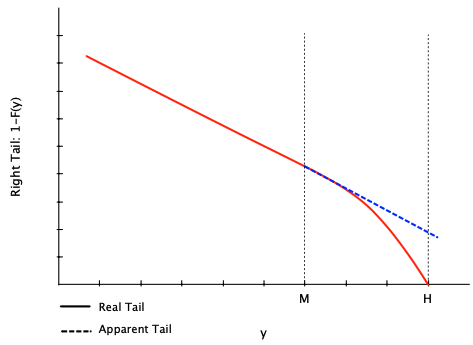
\includegraphics[width=1\linewidth]{images/taleb-limit-slimmed.png}\\
    \textit{Figure 15.1 from T19~\cite{taleb2019statistical} p.~279}
   \caption{As shown if you only
   observe a distribution up to some value M,
    you may be tempted to fit a line through the
   data (dotted blue line).
   But if there were in fact a limit to the distribution at H,
   you would be overestimating
   the true number of very extreme events (red curve),
   predicting events that were larger than were possible.}
   \label{fig:up-bound-taleb}
   \end{minipage}

   \begin{minipage}{0.45\textwidth}
   \centering
   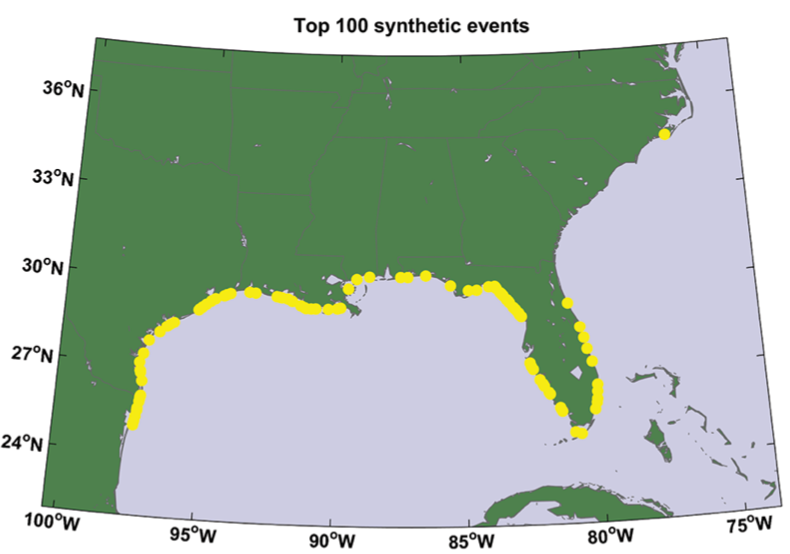
\includegraphics[width=1\linewidth]{images/top-100-landfalls.png}\\
   \textit{Figure 3b from \cite{emanuel2017will}}
   \caption{The top 100 most rapidly intensifying events in the model,
   showing that models capture far more of these TCs in the Gulf of Mexico
   and Florida than further north.
     }
   \label{fig:top-100}
   \end{minipage}
   \begin{minipage}{0.45\textwidth}
   \centering
   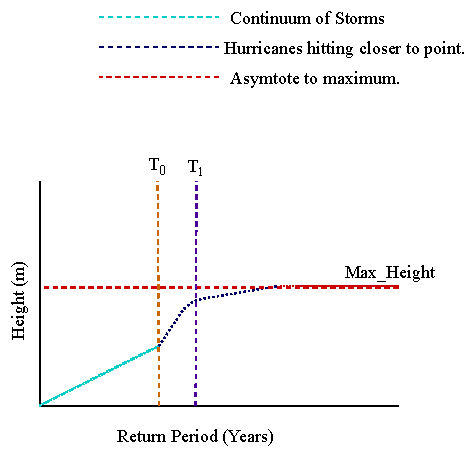
\includegraphics[width=1\linewidth]{images/Return_Hypothesis.pdf}
   \vspace{-15pt}
  \caption{The maximum height is a function of the potential intensity
  allowed by the climate, and the responsiveness of that point on the coastline to a
  wind stress of that size. If T$_0$, or T$_1$, is a similar or greater than the time period of
  measurement, then it is respectively possible that no hurricanes exist in the data sample,
  or that no hurricanes make direct landfall at that location.}
    \label{fig:return_hyp_new}
    \end{minipage}





\end{figure*}


\subsection{Comparison to POT GPD}
The other alternative is to use the peak-over-threshold method.
There are a number of alternatives as to how you should choose the
threshold.

\subsection{Enforcing an asymptote using potential intensity theory }
As noted in~§~\ref{sec:hurr-theory} there is some maximum size
that a tropical cyclone might be expected to be able to reach given
the climate. This gives us information as to the shape of the probability
distribution beyond what just curve-fitting the tail.

%\FloatBarrier
%
\section{Application of the Developed Model to Hindcasts and Forecasts}
\label{sec:6_Application}


\begin{itemize}
\item Problem.
\item Problem.
\item Observational Data.
\end{itemize}

\section{Discussion}
\label{sec:7_Discussion}

\label{sec:future}

Different models have varied systematic biases
and resolutions. We could measure how
the responsiveness changes as the resolution decreases. The value at 4km distance in
\texttt{tyr} (c.~1.6m) of Hurricane Katrina (see Figure~\ref{fig:katrina}),
is smaller than the value observed at the coast itself (c.~9m in places).
It must increase with a bound.
Combining the coastline outputs with a high resolution indundation model
would allow direct comparison with tidal gauges.
Data is available from tidal gauges worldwide~\cite{tadesse2020data, arns2020non},
and particularly for the US.\footnote{
However frequencies of the data are variable,
and the data extraction API is poorly designed.}

Models such as LLC4320~\cite{Abernathey2017}  include tides,
 despite computational expense,
introducing non-linear tide-surge interactions~\cite{
feng2019characteristics, arns2020non}.
Dangerous storm surges, e.g.~the 1938 New England
Hurricane, coincided with spring high tides.
As harm is a convex function T20~\cite{taleb2019statistical, Taleb2012AntifragileH},
this interaction will increase the hazard of storm surges.
According to Arns~et~al.~2020~\cite{arns2020non}
these effects are strongest on the E~UK,
E~US, and S~Japan coasts.

There are insufficient TCs in CMIP members~\cite{camargo2013global},
because the processes involved
in cyclogenesis are hard to resolve in climate models.
As is shown in Figure 19 of~\cite{williams2018met},
 for HadGEM3 this is particularly a problem in the North Atlantic~\cite{tomassini2017interaction}. % §~\ref{sec:cyclogenesis}.
CMIP members are colder in the tropics than observations~\cite{camargo2013global},
which may lead to less TCs.
For a recently published explanation see Seager et al.~2019~\cite{seager2019strengthening}.


TC PI theory is well supported,
but a few super-intense tropical cyclones have been observed~\cite{camargo2019tropical}.
This could be a result of treating the parameters $C_k$, $C_D$, as constant in the derivation (§~\ref{sec:param}).

The SSH does not reach its steady state as soon as
stress is applied, which this leads
to the regression being distorted by hysteresis.
It would therefore make sense to give the ML algorithm
a series of previous $\eta$ values for different lags.


%\subsection{Summary of systematic errors}
\label{sec:sys-errors}
Table~\ref{tab:syst_error} shows the list of systematic errors that effect the
observed hazard, most of which will lead to an underestimate.

\begin{table}[ht]
\resizebox{\columnwidth}{!}{%
\begin{tabular}{l L{8.5cm}}
%\hline \hline
\textbf{Effect} & \textbf{Source}\\
\hline
($-$) & Coarsening of time to daily outputs.\\
($-$) & Lack of cyclogenesis  $\implies$ not enough
        TCs~\cite{tomassini2017interaction, williams2018met, FurtherInfo}.\\
($\pm$) & Parameterisation of heat transfer $\implies$ wrong TC strength.\\
($\pm$) & Parameterisation of wind stress $\implies$ wrong TC surge.\\
($-$) & SSH 4km out from the coast (centre of cell).\\
($-$) & No non-linear surge-tide interaction.\\
($-$) & Limited wave build up.\\
($-$) & Long TC return periods $> 100$~yrs (e.g.~New England).\\
($\pm$) & Inaccurate bathymetry.\\
\hline
\end{tabular}
}
\caption{Systematic sources of error for the estimate of TC-induced storm surge
hazard.}
\label{tab:syst_error}
\end{table}


\FloatBarrier
\section{Conclusion}
\label{sec:8_Conclusion}

Storm surges rise out of the sea due to the stress applied to the surface,
with their size dependent to the size of the stress above and
the slope of the bathymetry beneath.
This thesis should provide a basis for
future studies, as it radically reduces the computational cost
of training algorithms, choosing only the
land adjacent cells.

As set out, we could be able to combine the insights of
extreme value and TC potential intensity theories to allow
us to more accurately estimate the hazards posed to coastal communities
in the future.

%\FloatBarrier

%%%%%%%%%%%%----End Real Report---%%%%%%%%%%%%%%%%%%%

%%TC:ignore
\FloatBarrier
\footnotesize
\printbibliography
\normalsize
%%%%%%%%%%%----Start Appendices---%%%%%%%%%%%%%%%%%%%%%
\appendix
\section{Acknowledgements}
Dr.\ Dan Jones (British Antarctic Survey) has been an invaluable help throughout this project.
Dr.\ Laure Zanna (New York University) was a useful counsel as to what is feasible,
 and what the common views in the literature were.
Dr.\ Pierre Mathiot (Met Office) also deserves my thanks for
producing the high-resolution ORCA12 data that I used, and
for answering my queries.
I also received advice from Dr.\ Rory Bingham (Bristol).
I hope that in the fullness of time these collaborators will be rewarded
as co-authors, as we expand and publish the
work begun here.

PRIMAVERA received funding from the European Union's Horizon 2020
Research and Innovation Programme under grant agreement no.~641727.


\section{Resources used}

This report was typeset in \LaTeX\
with \texttt{matplotlib}~\cite{Hunter:2007} and \texttt{draw.io}~\cite{DrawIO}
for original figures, WebPlotDigitiser for data extraction~\cite{WebPlotDigitiser},
and Mathpix for maths extraction~\cite{mathpix}.
It makes extensive uses of the \texttt{sklearn} library~\cite{scikit-learn} as highlighted in the report.
The \texttt{cmocean} package~\cite{thyng2016true}\footnote{\url{https://matplotlib.org/cmocean/}}
provided oceanography standard colour maps, \texttt{numba.jit}~\cite{lam2015numba} for speed,
\texttt{xarray}~\cite{hoyer2017xarray} for ND~data.
I used Panolpy and \texttt{ncview}\footnote{\url{http://meteora.ucsd.edu/~pierce/ncview_home_page.html}}
for inspecting NetCDF files.

I made use of these textbooks:~\cite{roisin2010GFD,williams2011ocean,ITILA,
sivia2006data,williams2006gaussian,
}.\footnote{\url{http://www.gaussianprocess.org/gpml/chapters/RW.pdf
}}
I found Stephen Pinker's book~\cite{pinker2015sense} especially useful and entertaining.
Any errors in writing are my own, but this book does defend the selective use of the
passive voice, if either its presence or absence in certain sections frustrates the reader.
I felt more comfortable with directly talking about cause after reading
Judea Pearl's \textit{The Book of Why}~\cite{pearl2018book}.

The code listing for this report is available as a \texttt{python3} repository on Gitlab~\cite{gitlab, skextremes}.
 I have tried to write using PEP8 style\footnote{\url{https://www.python.org/dev/peps/pep-0008/}}
 and have been helped by \texttt{pylint} and Pycharm.\footnote{\url{https://www.jetbrains.com/pycharm/download/}}
 Errors are dealt with as per the Physics formula booklet~\cite{MathsFormulaBooklet}
 by the \texttt{python3.uncertainties}
 package~\cite{lebigot2010uncertainties}.\footnote{\url{https://pythonhosted.org/uncertainties/}}

 To move and process the large quantity of climate data on the HPCs I used \texttt{tmux}
 to run \texttt{bash}, \texttt{python3}, and \texttt{fortran} scripts.

\section{Supplementary results}
\label{sec:sup-res.}

\subsection{Summary variable statistics}
\label{sec:sum-var-stat}
Figures~\ref{fig:tauuo_stats_america}~&~\ref{fig:tauvo_stats_america} which
are analogous to Figure~\ref{fig:ssh_stats_america}, but for $\tau_u$ and
$\tau_v$.

\begin{figure*}[htb!]
    \centering
    \includegraphics[width=0.6\linewidth]{../surge/plots/stats_points_plottauuo.pdf}
       \hspace{0pt} \includegraphics[width=0.285\linewidth]{../surge/plots/stats_points_plottauuo_1.pdf}
    \vspace{-7pt}
    \caption{\texttt{tauuo}, $\tau_u$ for \texttt{tyr}, \texttt{eUS}}
   \label{fig:tauuo_stats_america}

   \includegraphics[width=0.6\linewidth]{../surge/plots/stats_points_plottauvo.pdf}
      \hspace{0pt} \includegraphics[width=0.285\linewidth]{../surge/plots/stats_points_plottauvo_1.pdf}
   \vspace{-7pt}
   \caption{\texttt{tauvo}, $\tau_v$ for \texttt{tyr}, \texttt{eUS}}
  \label{fig:tauvo_stats_america}
\end{figure*}


\begin{figure*}[htb!]
    \centering
    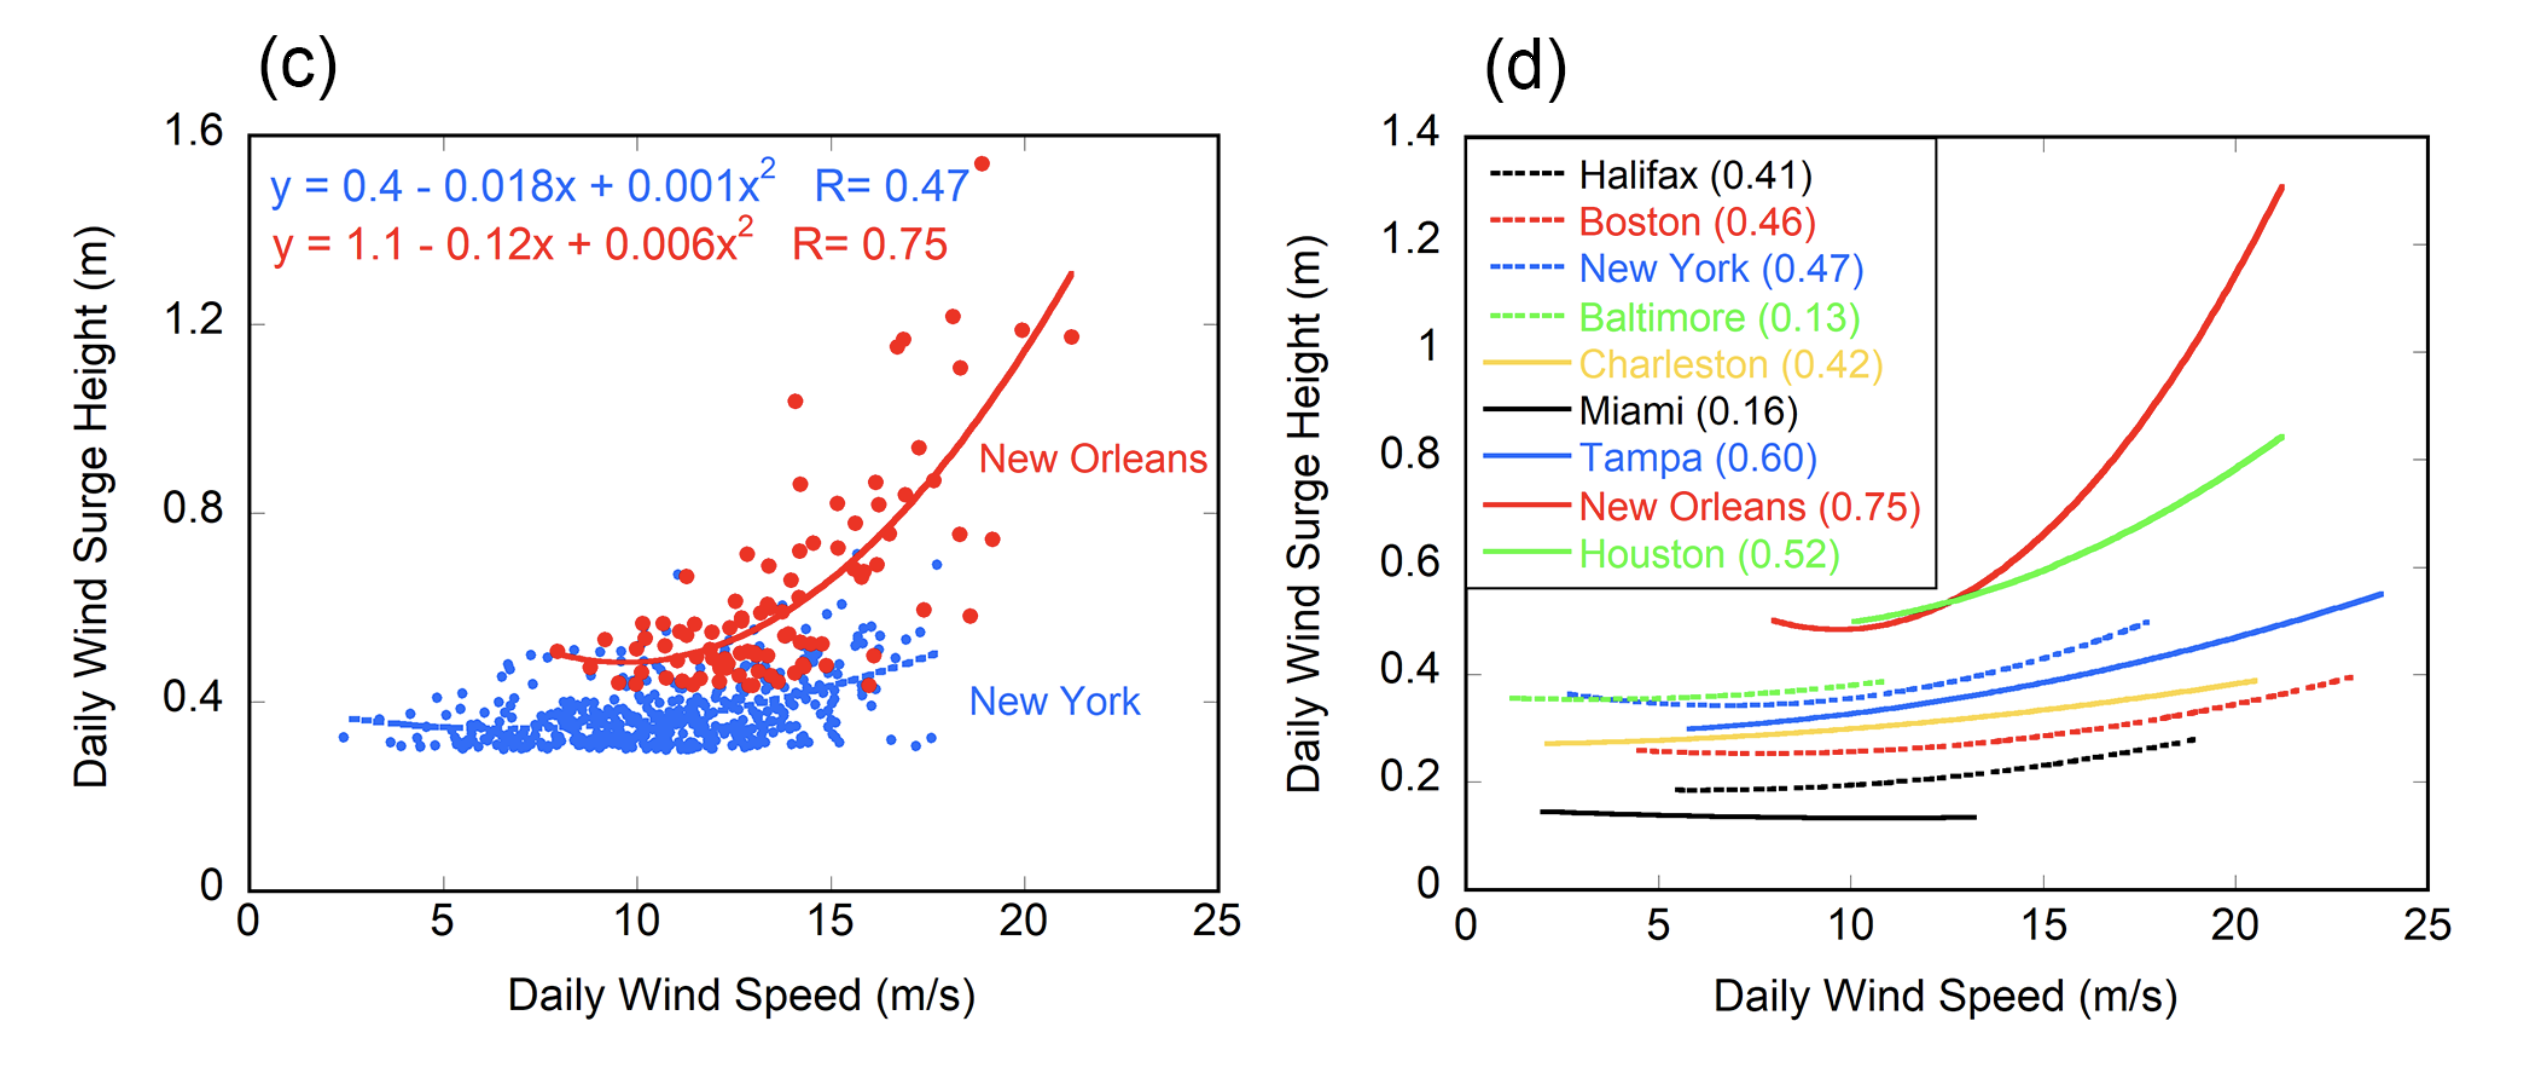
\includegraphics[width=0.8\linewidth]{images/example-images/yin-responsiveness.png}
    \vspace{-7pt}
    \caption{Figure 10c \& 10d in Yin et al.~2020~\cite{ZannaPreprint}. }
   \label{fig:yin-responsiveness}

   \includegraphics[width=0.8\linewidth]{../surge/plots/score-plot/score_plot.pdf}
   \vspace{-7pt}
   \caption{Linear Regression of $ \Delta \eta$ against $|U|^2$ for $ \Delta\eta>0$.
   Only generalises for the most vulnerable points. Most variance not modelled.}
  \label{fig:simple-responsiveness-results}
\end{figure*}


\paragraph{Gaussian processes (GPs)}
\begin{itemize}
\item Equations 2.13-2.14 in GPML~\cite{williams2006gaussian}.
\begin{align}
m(\mathbf{x})&=&\mathbb{E}[f(\mathbf{x})] % \tag{Mean}
\\
k\left(\mathbf{x}, \mathbf{x}^{\prime}\right)&=&\mathbb{E}
\left[(f(\mathbf{x})-m(\mathbf{x}))\left(f\left(\mathbf{x}^{\prime}\right)
-m\left(\mathbf{x}^{\prime}\right)\right)\right]
%\tag{Covariance}
\\
f(\mathbf{x})& \sim& \mathcal{G} \mathcal{P}\left(m(\mathbf{x}),
 k\left(\mathbf{x}, \mathbf{x}^{\prime}\right)\right)%\tag{GP}
\end{align}
\item Can assume $m(\mathbf{x})=0$ without terrible consequences.
 \item Thought should be put into the form of $k\left(\mathbf{x},
  \mathbf{x}^{\prime}\right)$~\cite{duvenaud2014automatic}.
\item GPs assume that there is a Gaussian error around each point,
      but this is often not the case in real variables.
      However, it is often possible to transform to
      a space where this is the case, Krige there,
      and then transform
      back~\cite{snelson2004warped}.\footnote{\url{http://mlg.eng.cam.ac.uk/zoubin/papers/gpwarp.pdf}}
      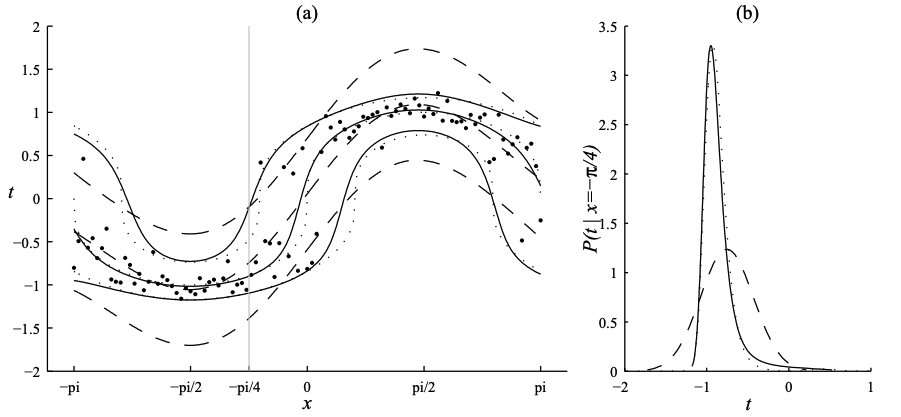
\includegraphics[width=\linewidth]{images/example-images/warped-example.png}\\
      \textit{Figure 1 from~\cite{snelson2004warped}}
\item Lewis Fry Richardson (1948) showed that the estimates
      of deaths during a war had
      symmetric error bars in logarithmic space~\cite{richardson1948variation}.
      \cite{snelson2004warped}~mentions this as a common trick.
 \end{itemize}

\begin{figure*}[htb!]
    \centering
    \includegraphics[width=0.85\linewidth]{../surge/plots/stats_points_plot_2.pdf}
    \vspace{-7pt}
    \caption{An attempt to check whether there are discontinuities
     over the special points, to explain the offsets of the means.
     The points are ordered from Eastport (EP) (furthest north east),
     to Rockport (RP) (furthest south west). From the plot it is visible
     that there is a low frequency annual component to each signal, and that
     the excursions are more common during autumn and winter, with
     relative calm in spring.}
    \label{fig:individual_zos}
    \includegraphics[width=0.85\linewidth]{../surge/plots/ahh/ahhhhh4.pdf}
    \vspace{-7pt}
    \caption{Mean SSH over points of the US coast over the two year period. There is a strong yearly periodicity in $\eta$ (and its variance?).
     Kriged with a Sobol quasirandom subsample~\cite{sobol1967distribution} of 6000 time points.
     }
    \label{fig:gauss-mean}
\end{figure*}

\begin{figure}[htb!]
\includegraphics[width=\linewidth]{../surge/plots/vc_bath_list.pdf}
\vspace{-25pt}

\caption{Isobaths plotted for \texttt{vc}.}
\label{fig:bath}
\includegraphics[width=\linewidth]{../surge/plots/vc_distance_isobath.pdf}
\vspace{-25pt}

\caption{Distance to isobaths from points on \texttt{vc}.}
\label{fig:vc_isobath}
\includegraphics[width=\linewidth]{../surge/plots/vc_isobath_correlate.pdf}
\vspace{-25pt}

\caption{The correlation matrix between the different isobath's distance's to
\texttt{vc}.}
\label{fig:vc_isobath}
\end{figure}


\begin{figure}[htb!]
\centering
\includegraphics[width=\linewidth]{../surge/plots/vc_angle_heatmap.pdf}
\caption{Normal bearing, $B^{\prime}$, along \texttt{vc}.

         }
\label{fig:angle_heatmap}

\includegraphics[width=\linewidth]{../surge/plots/vc_derivative_heatmap.pdf}
\caption{Convexity metric along \texttt{vc}.
         The three panels above show bay like concavity in blue, and convexity
         in red. At the largest $\sigma$ only the largest headlands visible (C), whereas the smallest bays are visible at a lower
        $\sigma$ (A).
}
\label{fig:derivative}
\end{figure}


\FloatBarrier

\section{Reference Theory}
\label{sec:ref-theory}
This section draws heavily form~\cite{roisin2010GFD}.

\subsection{Basic Oceanographic Equations}

The Coriolis parameter $f$ is given by
\begin{equation}
f=2 \Omega \sin \varphi,
\label{eq:coriolis}
\end{equation}
where $\varphi$ is the latitude of the position and $\Omega$ is the angular
 frequency of the Earth's rotation.

\subsubsection{Basic Fluid Mechanics}
Fluid mechanics is based on three simple equations~\cite{landau1959course}:
 The conservation of matter,
\begin{equation}
\frac{\partial \rho}{\partial t} + \boldsymbol{\nabla}(\rho \boldsymbol{u}) = 0,
\tag{Matter}
\label{eq:Matter}
\end{equation}
the conservation of momentum,
\begin{equation}
\rho\left (\frac{\partial \mathbf{u}}{\partial t}
+ \mathbf{u}(\boldsymbol{\nabla}\cdot \mathbf{u})\right) =
- \boldsymbol{\nabla}P + \boldsymbol{\nabla}\cdot \underline{\underline{\tau}}
- \rho\boldsymbol{\nabla}\phi,
\tag{Momentum}
\end{equation}
and the conservation of energy,
\begin{equation}
\begin{array}{l}
\rho \left( \frac{\partial h}{\partial t} + \boldsymbol{\nabla}
\cdot (h\mathbf{u})\right) = \\ \quad\quad- \left( \frac{\partial P}{\partial t}
+ \mathbf{u}\cdot (\boldsymbol{\nabla} P) \right)
+ \boldsymbol{\nabla}\cdot (k \boldsymbol{\nabla} T )
+ (\underline{\underline{\tau}}\cdot\boldsymbol{\nabla})\mathbf{u}.\end{array}
\tag{Energy}
\end{equation}
Where we have assumed that we are in an inertial frame and the variables are
labelled as in Table~\ref{tab:fluid_variables}.

\begin{table}[h!]
    \centering
    \begin{tabular}{ll}
        $\rho$ & Density. \\
        $t$ & Time. \\
        $\mathbf{u}$ & Velocity. \\
        $P$ & Pressure. \\
        $\underline{\underline{\tau}}$ & Deviatronic stress (2nd order tensor). \\
        $\phi$ & Gravitational potential. \\
         $h$ & Enthalpy.\\
         $T$ & Temperature. \\
         $k$ & Thermal conductivity.\\
         $c_p$ & Heat capacity.\\
         $\eta$ & Viscosity. \\
         $H$ & Heat production density.\\
    \end{tabular}
    \caption{Symbols for fluid mechanical equations.}
    \label{tab:fluid_variables}
\end{table}

\subsubsection{Boussenesq Approximation}
We can also normally assume that all density variations can be ignored that
 are not on the gravitational term (the Boussenesq approximation),
  which simplifies the equations considerably as Equation~\ref{eq:Matter} becomes
\begin{equation}
    \boldsymbol{\nabla}\cdot\mathbf{u} = 0, \tag{B-Matter}
\end{equation}
and we also could derive that
\begin{equation}
\rho\left (\frac{\partial \mathbf{u}}{\partial t}
+ \mathbf{u}(\boldsymbol{\nabla}\cdot \mathbf{u})\right)=
-\nabla P+\eta \nabla^{2} \mathbf{u}-\rho \boldsymbol{\nabla}\phi, \tag{B-Momentum}
\end{equation}
\begin{equation}
\rho c_{p}\left(\frac{\partial T}{\partial t}
+\mathbf{u} \cdot \nabla T\right)=k \nabla^{2} T+\rho H. \tag{B-Energy}
\end{equation}

\subsubsection{Extension to a Rotating Sphere}
\label{app:rotating_equations}
However the surface of the Earth reference frames rotate,
 which makes these equations less elegant.
  The final form of the equations in an earth bound reference frame
  is found by applying the identity
\begin{equation}
\frac{\mathrm{d}}{\mathrm{d} t} \boldsymbol{A}=
\left[\left(\frac{\mathrm{d}}{\mathrm{d} t}\right)_{r}
+\mathbf{\Omega} \times\right] \boldsymbol{A},
\end{equation}
for converting to a rotating reference frame to the previous equations.
\begin{equation}
\begin{array}{l}
\rho \frac{D \mathbf{u}}{D t}=\\\quad\quad-\boldsymbol{\nabla} P+
\eta \nabla^{2} \mathbf{u}+\frac{1}{3} \eta \nabla(\nabla \cdot \mathbf{u})
+\rho \mathbf{g}\\\quad\quad-\rho\left(2 \mathbf{\Omega} \times \mathbf{u}
+\mathbf{\Omega} \times(\mathbf{\Omega} \times \mathbf{x})
+\frac{d \mathbf{u}}{d t}\right)\end{array}.
\tag{R-Momentum}
\end{equation}

\subsubsection{The Ekman Spiral}

Due to the effects introduced in \cref{app:rotating_equations},
the wind does not simply cause the water to go in
the same direction~\cite{ekman1905influence}.
Instead, in the northern Hemisphere,
 the surface travels c.~45 degrees to the
right of the prevailing wind, and each subsequent
layer of the water travels to the right of that.
If the water column is deep enough, with
assumptions about the friction coefficients of the water column,
the net transport is 90 degrees to the right of the prevailing wind
(see Figure~\ref{fig:ekman}).\footnote{\url{https://oceanservice.noaa.gov/education/kits/currents/media/supp_cur05e.html}}

\begin{figure}
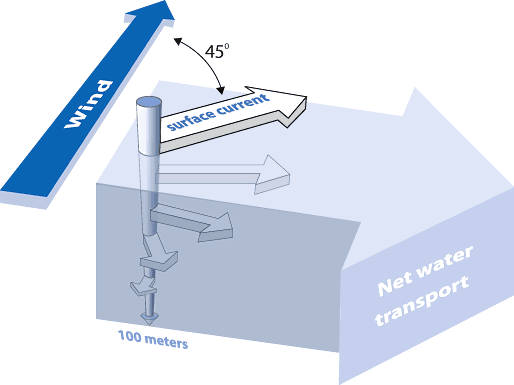
\includegraphics[width=\linewidth]{images/ekman_spiral.png}
\caption{The Ekman spiral.}
\label{fig:ekman}
\end{figure}



\subsubsection{Shallow Water Equations}
\label{sec:shallow_equation}

\begin{itemize}
    \item The shallow water equations are simply:
    \begin{eqnarray}
     -\left(\frac{Du}{Dt} + \underline{f}\times\underline{u} \right) &=& g \underline{\nabla} \eta  \\
 \frac{Dh}{Dt} + h \underline{\nabla}\cdot\underline{u} &=& 0\\
\Leftrightarrow  \;\quad\quad\quad\quad \frac{\partial h}{\partial t} + \underline{\nabla}\cdot (h\underline{u})&=& 0 \\
w. \;\quad\quad \eta(x, y, t) - \eta_{b}(x, y)  &=& h \\
\& \quad\quad\quad\quad\quad\quad \frac{\partial}{\partial t} + \underline{u}\cdot\underline{\nabla}   &=& \frac{D}{Dt}
    \end{eqnarray}
\end{itemize}


\subsection{Simple Tropical Cyclone Models}

\subsubsection{Introduction to azimuthally symmetric models}
One of the dominant controls on storm surge events on the Eastern Seaboard
 of the US are the large tropical cyclones (Hurricanes).
  These large vortices can be surprisingly well modelled by azimuthally
   symmetric analytic pressure distributions, and the velocity distribution
    that would be expected to result from them.

\subsubsection{Holland Hurricane Model}
The most prominent is the  Holland model~\cite{holland1980analytic,holland2010revised}
 which elaborated on a class of functions initially proposed
 by Schloemer 1954~\cite{schloemer1954analysis}.
  This model uses the dimensionless pressure \( P^{\prime}\) given by

\begin{equation}
    P^{\prime}=\dfrac{P-P_{c}}{P_{n}-P_{c}},
\end{equation}
where $P_c$ is the pressure at the centre of the storm, and $P_n$ is
the ambient pressure, ideally at at an infinite distance from the storm.
They then define the pressure relation
\begin{equation}
    r^{B}\ln(\frac{1}{P^{\prime}})=A,
\end{equation}or in a more elegant form
\begin{equation}
P^{\prime}=\exp{(-\frac{A}{r^B})},
\end{equation}
where A and B are model parameters which must be found empirically.

In steady state around this  pressure distribution generally yields a
 velocity~\cite{roisin2010GFD} of:
\begin{equation}
    U_g = \sqrt{AB(P_{n} - P_{c})\frac{\exp{(-\frac{A}{r^{B}})}}{\rho r^{B}}
     +\frac{r^2f^2}{4}}-\frac{rf}{2}.
\end{equation}
If we assume that the eye of the TC itself is small s.t. the Coriolis force
 is much smaller than the centrifugal then we can approximate this as

\begin{equation}
U_c = \sqrt{AB(P_{n}-P_{c})\frac{\exp{(-A/r^{B})}}{\rho r^{B}}}.
\end{equation}
The maximum velocity
\begin{equation}
U_m = (\frac{B}{\rho e})^{0.5}(P_n-P_c)^{0.5},
\end{equation}
which occurs at
\begin{equation}
R_m = A^{1/B}.
\end{equation}
There are at least two degrees of freedom:
B defines the height of the peak and A determines its relative position.
 The difference between the ambient and central pressure of the vortex still
 enter into the velocity expression, so there are four degrees of freedom when
  those are included.


\subsubsection{The Rankine Vortex}

The Rankine vortex is
\begin{equation}
C=\left\{\begin{array}{ll}U \frac{R_m}{ r}& \text{ if } r < R_m,\\
U\frac{r}{ R_m} & {\text { if } r>R_m},
\end{array}\right.
\end{equation}
where C is a constant, and the two sections are joined together
 so that the velocity is continuous at the boundary.
   The two degrees of freedom are $R_m$ and C.
This can be modified to a more general relation where $Ur^{x}=\text{constant}$
where X is a new parameter to fit,
which lies between 0.4 and 0.6~\cite{holland1980analytic}.


\subsection{Moist thermodynamics}
\label{sec:moist-thermodynamics}

The law of thermodynamics for a PV system is,

\begin{equation}
d U=T d S-P d V,
\end{equation}

which can be adapted to the moist form, as in
Appendix 1 Emanuel 1986~\cite{emanuel1986air}.

\begin{equation}
T d s^{*}=d u+p d \alpha-L d q^{*}
\end{equation}

where $u$ isn the internal energy, $L$ is the heat of vaporisation,
and $q^{*}$ is the saturation mixing ration.
We also define the saturated  moist enthalpy,

\begin{equation}
h^{*} \equiv u+p \alpha-L q^{*},
\end{equation}

and can therefore show that,

\begin{equation}
d h^{*}=T d s^{*}+\alpha d p.
\end{equation}

This implies that,

\begin{equation}
\begin{array}{l}
\left(\partial h^{*} / \partial p\right)_{s^{*}}=\alpha, \\
\left(\partial h^{*} / \partial s^{*}\right)_{p}=T,
\end{array}
\end{equation}

As $q^{*}$ is only a function of temperature and pressure,
$h^{*}$ is a state variable. Therefore it is a function of
any of other two state variables. For $p$ and $s^{*}$,

\begin{equation}
\left(\frac{\partial}{\partial s^{*}}\right)_{p}\left(\frac{\partial h^{*}}{\partial p}\right)_{s^{*}}=\left(\frac{\partial}{\partial p}\right)_{s^{*}}\left(\frac{\partial h^{*}}{\partial s^{*}}\right)_{p},
\end{equation}

which implies,

\begin{equation}
\left(\frac{\partial \alpha}{\partial s^{*}}\right)_{p}=\left(\frac{\partial T}{\partial p}\right)_{s^{*}}.
\end{equation}

\paragraph{Tropical cyclone derivation}

From Section 3 Emanuel 1986~\cite{emanuel1986air}.
Air rushes inwards along the isotherm from $r_{0}$ acquiring
incremental latent heat

\begin{equation}
\Delta Q_{1}=\int_{\theta_{e a}}^{\theta_{e}} C_{p} T_{B} d \ln \theta_{e}=C_{p} T_{B} \ln \frac{\theta_{e}}{\theta_{e a}},
\end{equation}

Where $\theta_{e a}$ is the equivalent potential temperature at
$r_{0}$. The air ascends at constant entropy to the lower stratosphere
at a large radius. The air loses enough total heat through radiation cooling
to return to ambient temperature $\theta_{e}$ so

\begin{equation}
\Delta Q_{2}=\int_{\theta_{e}}^{\theta_{a a}} C_{p} T_{\mathrm{out}} d \ln \theta_{e}=-C_{p} \bar{T}_{\mathrm{out}} \ln \frac{\theta_{e}}{\theta_{e a}},
\end{equation}

where $\bar{T}_{\mathrm{out}}$ is given by,

\begin{equation}
\bar{T}_{\mathrm{out}} \equiv \frac{1}{\ln \theta_{e}^{*} / \theta_{e a}} \int_{\mathrm{ln} \theta_{e a}}^{\ln \theta_{e}} T_{\mathrm{out}} d \ln \theta_{e}^{*}.
\end{equation}

the total heating is therefore

\begin{equation}
\Delta Q=\Delta Q_{1}+\Delta Q_{2}=C_{p} T_{B} \epsilon \ln \frac{\theta_{e}}{\theta_{e a}},
\end{equation}

where 
$
\epsilon \equiv\left(T_{B}-s\bar{T}_{\text {out }}\right) / T_{B}
$
is the thermodynamic efficiency and $T_b$ is the temperature at the top of the
boundary layer. By the first law of thermodynamics, the total heating
must balance the work done,

\begin{equation}
\Delta Q=W_{P B L}+W_{0}
\end{equation}

where $W_{PBL}$ and $W_0$ are the work done in the boundary layer and outflow
respectively. $W_0$ is proportional to the kinetic energy required to
bring the angular momentum of the outflow back to the ambient value:

\begin{equation}
\begin{aligned}
W_{0} &=\frac{1}{2} \Delta V^{2}=\frac{1}{2}\left[\left(\frac{M}{r_{1}}
-\frac{1}{2} f r_{1}\right)^{2}-\left(\frac{M_{0}}{r_{1}}-\frac{1}{2} f r_{1}\right)^{2}\right] \\
&=\frac{1}{2}\left[\frac{M^{2}-M_{0}^{2}}{r_{1}^{2}}+f\left(M_{0}-M\right)\right]
\end{aligned}
\end{equation}

where we have used,

\begin{equation}
M \equiv r V+\frac{1}{2} f r^{2}
\end{equation}

where $r_1$ is the large radius at which the exchange place, so that,

\begin{equation}
\lim _{r_{1} \rightarrow \infty} W_{0}=\frac{1}{2} f\left(M_{0}-M\right)=\frac{1}{4} f^{2}\left(r_{0}^{2}-r^{2}\right)-\frac{1}{2} f r V.
\end{equation}

Which can be then used to infer the work done in the boundary layer:

\begin{equation}
W_{\mathrm{PBL}}=C_{p} T_{B} \epsilon \ln \frac{\theta_{e}}{\theta_{e a}}+\frac{1}{2} f r V-\frac{1}{4} f^{2}\left(r_{0}^{2}-r^{2}\right)
\end{equation}


we can then use Bernoulli's equation,

\begin{equation}
p+\frac{1}{2} \rho V^{2}+\rho g h=\text { constant },
\end{equation}

and the Exner function is used in place of pressure:

\begin{equation}
\pi=\left(p / p_{0}\right)^{R / C_{p}}.
\end{equation}

where $C_p$ is the heat capacity at constant pressure,
$p_{0}$ is the ambient pressure, to see that,

\begin{equation}
\frac{1}{2}
V^{2}+C_{p} T_{B} \ln \pi+W_{\mathrm{PBL}}=0 \quad \text { at } \quad z=0.
\end{equation}


Using the gradient wind equation,

\begin{equation}
\alpha \frac{\partial p}{\partial r}=\frac{V^{2}}{r}+f V=\frac{M^{2}}{r^{3}}-\frac{1}{4} f^{2} r
\end{equation}

an expression for the pressure is then,

\begin{equation}
\begin{array}{r}
\ln \pi+\frac{1}{2} r \frac{\partial \ln \pi}{\partial r}+\epsilon \ln \frac{\theta_{e}}{\theta_{e a}}-\frac{1}{4} \frac{f^{2}}{C_{p} T_{B}}\left(r_{0}^{2}-r^{2}\right)=0 \\
\text { at } z=0
\end{array}
\end{equation}

There is a further correction term decreasing the central pressure,
created by removing angular momentum and heat at finite $r_1$
rather than the limit as $r_1\to\infty$:

\begin{equation}
\delta \ln \pi=\frac{-\frac{1}{8} \frac{f^{2} r_{0}^{4}}{r_{1}^{2}}}{C_{p} T_{B}\left[1-\epsilon\left(1+\frac{L q_{a}^{*} \mathrm{RH}_{s}}{R T_{s}}\right)\right]},
\end{equation}

which is insignificant when $r_1=r_0$, and only important if $r_0$ is very large.



\begin{table}[h!]
\centering
\begin{tabular}{lll}
\hline \hline
\textbf{Quantity} & \textbf{Scale} & \textbf{Typically c.}\\
\hline
Length & $\chi_s^{1/2}f^{-1}$ & 1000 km \\
Time & $C_D^{-1}H\chi_{s}^{-1/2}$ & 16 hr \\
Azimuthal velocity & $\chi_s^{1/2}$ & 60 m s$^{-1}$\\
Radial velocity & $\frac{1}{2}C_d\chi_s f^{-1}H^{-1}$ & 10 m s$-1$\\
Vertical velocity & $C_D \chi_s^{1/2}$ & 6 cm s$-1$\\
\hline \hline
\end{tabular}\\
\textit{Table 1 from~\cite{emanuel1991theory}.}
\caption{The different scales within a tropical cyclone (TC).
$\chi_s\equiv(T_s-T_t)(s_{0}^{*}-s_a)$, the thermodynamic disequilibrium parameter,
 where $T_s$ is the temperature
of the ocean,$T_t$ is the ambient temperature of the tropopause,
$s_{0}^{*}$ is the saturation entropy of the ocean surface and
$s_a$ is the entropy of the normal tropical atmosphere near sea level.
$s_{0}^{*}-s_a$ represents the thermodynamic disequilibrium of the ocean-atmosphere
system. $H\equiv$ depth of convecting layer, $f\equiv$ twice the
local vertical component of Earth's angular velocity, $C_D\equiv$
dimensionless exchange coefficient.}

\label{tab:hurr-scales}
\end{table}



\onecolumn
\section{Repositories}
To reproduce the work in this report, it should be possible to just run these
commands in terminal:

\begin{verbatim}
> git clone https://gitlab.com/sdat2/surge.git

> git clone https://github.com/sdat2/scikit-extremes.git

\end{verbatim}

and then follow the instructions in the \texttt{surge} README file.

\subsection{\texttt{surge} repository}

My primary code git repository is called `\texttt{surge}'~\cite{gitlab}.
It is quite large (see below), and I do not think that it would be helpful to reproduce any of the code here
as the logical structure of any interesting code is represented by the
algorithms included in the report. There are so many lines of code within the file
repository as shown below, and I think the easiest way to understand it would be to open
and run the repository in an appropriate development environment rather than a pdf file.
The repository comes with the slimmed down point data files for the american and
viet-chinese coast, and all of the results in this report could be reproduced from them.
This repository was developed from scratch by myself during this academic year 2019-20.
There are a couple of files that I borrowed from others who were
experienced with using the HPC (e.g. bash batch job file).


\verbatiminput{../surge/environment/cloc.txt}

Below is the README of the \texttt{surge} repository which is designed to
introduce the project and give instructions to replicate the results:

\verbatiminput{../surge/README.md}

\subsection{\texttt{scikit-extremes} repository}

To implement models from univariate extreme value theory, I built
on an unfinished repository that I locally installed from github,
called \texttt{scikit-extremes}~\cite{skextremes}.

\verbatiminput{../scikit-extremes/cloc.txt}

\subsection{\texttt{report} repository}

I wrote the report and presentations in \LaTeX.

\verbatiminput{appendices/cloc.txt}



\subsection{Dead Ends}

\begin{quote}
``I have not failed. I've just found 10,000 ways that won't work.''
Thomas Edison
\end{quote}

Initially I was quite convinced that it would be relatively
simple to apply the algorithms that my peers where applying
(Gaussian Processes) to this new problem~\cite{LeMaitre2019gaussian}, but I did not
forsee all of the technical problems that would be in the way of that.
Although it would have been possible to regress $\tau_u$, $\tau_v$ against
$\eta$ using Gaussian processes, and this would have been bound to produce a
higher $r^2$ value than linear regression because of the increased number of
degrees of freedom, it would have been impossible to give all of the points,
there is no simple way of summarising what the kernel contains,
and it would have taken many hours on the HPC to process the coastline.

One other thing that influenced my de-prioritisation of this
avenue was reading Taleb's \textit{The Black Swan}~\cite{taleb2007black} during Lent
term, which included extensive criticism of using Gaussian based methods in the
real world, particularly for the estimation of risk.
I also attended a Gaussian Processes Cambridge meetup where a practitioner noted that
Gaussian processes do not naturally cope well with extreme
events. This lead me to T19~\cite{taleb2019statistical} and using extreme value
theory with a greater amount of data using \texttt{control-1950}.
It does not rule out that using warped Gaussian processes, approximated as
warped SDEs, will not patch over these deficiencies in the future.

When I initially began to look at the ORCA12 output,
I thought that it would be easier to go from that 2D
curvilinear grid, to a rectilinear lat-lon grid before
I began to interpret the data. It was not obvious how
this was to be done, and so I asked Dr.~Mathiot, who recommended
I use SOSIE \texttt{fortran} package for interpolation.\footnote{\url{https://github.com/sdat2/sosie}}
The package was eventually coerced into working on my laptop and the JASMIN
HPC after I had run some example \texttt{fortran}
code\footnote{\url{https://gitlab.com/sdat2/fortran-examples}} on my laptop
to get my head round the language. It was only after this introduction to
the new language that I realised that interpolating the results was
unnecessary, and that it would probably lead to artefacts in the product as coastal
locations inherit the mask of the adjacent land.

I used \texttt{iris} to verify that the deformation of the ORCA12 grid was quite small
for all of the points that I initially chose (from the East~US coastline).

\paragraph{The MOOSE problems}

The \texttt{two-year} run was stored on the
Met Office's tape's.
To access the \texttt{two-year} run I used the
MASS transfer system on the JASMIN HPC.
During the first week and a half this system broke
with no restart after about 4GB of file transfer,
which meant that only the smallest files could be
moved to the group workspace. This seemed to magically resolve
itself the night before my second project meeting.
Originally, I was also not using \texttt{screen}
and therefore there was the additional failure-mode
that the wifi access from BAS to JASMIN would break,
thus halting the transfers to the group work space,
with no way to restart, except from the beginning.


\section{Wordcount}
The word limit for this thesis was 5000 words
(excluding abstract, figure captions, references, and appendices).
For full transparency, this is the full automatic breakdown:
\wordcount
%%TC:endignore
\fi


%%%%%%%%%%%%---End of Document---%%%%%%%%%%%%%%%%%%%%
\end{document}
